% !TeX spellcheck = da_DK
\section{Apopleksi}
Apopleksi er en sygdom, som har indvirkning på blodgennemstrømningen til encephalon, da den nedsætter blodtilførslen enten ved en blodprop eller en blødning \cite{Hjernesagen2015a}. Encephalon har brug for ilt og næringsstoffer for at kunne fungere normalt og er derfor afhængig af en konstant blodtilstrømning. Hvis tilstrømningen begrænses, kan det have alvorlige konsekvenser, da nervecellerne i encephalon skades efter få minutter pga. iltmangel eller kan i værste tilfælde gå tabt efter denne periode. \cite{Hjernesagen2015a,Schulze2011,Giraldo2015} Tidspunktet for forekomsten af symptomer, efter apopleksien er opstået, kan variere fra et par minutter til et par dage \cite{Kruuse2014,Academic2015}. Sundhedsstyrelsen definerer apopleksi som: "(...) pludseligt opståede fokalneurologiske symptomer af formodet vaskulær genese med en varighed på over $24$ timer" \cite{Sundhedsstyrelsen2009}. Hvis varigheden er under $24$ timer, betegnes det som transitorisk cerebral iskæmi (TCI), hvor de fleste tilfælde varer under en time uden permanent hjerneskade \cite{Sundhed.dk2014, Ritter2015}. Hvert år oplever flere tusinde danskere TCI, men det er sjældent, at de selv er bevidste herom. Symptomerne er milde og kan være en følelsesløshed i lemmerne eller i ansigtet samt korte oplevelser af forvirring, synsforstyrrelser og sproglige forstyrrelser. Det er sjældent, at der opstår følger fra TCI og derfor kræves der oftest ingen behandling. \cite{Hjernesagen2015a,Academic2015} 
%Symptomerne heraf er meget milde, og selvom man ikke får behandling for disse forbigående blodpropper i hjernen, er det sjældent, at der opstår mén fra tilfældet. [7]  
%Derudover kan der opstå mere alvorlige tilfælde af apopleksi, hvor det i værste tilfælde vil føre til koma eller død [11].
Risikofaktorer, der kan medføre apopleksi, er forhøjet blodtryk, rygning, højt kolesteroltal, diabetes og arvelige defekter. Konsekvenserne fra apopleksi kan omfatte forbigående eller varig lammelse af forskellige kropsdele, %på en eller begge sider af kroppen, 
vanskeligheder ved at tale og spise samt et tab i muskulær koordinering. \cite{Academic2015} En hurtig behandling er essentiel for at mindske disse konsekvenser \cite{Hjernesagen2015a}. \\ %Hver fjerde apopleksi patient er imidlertid afhængig af andres hjælp i hverdagen. \\ %(døde dele af hjernevæv)
Et apopleksitilfælde kan være forårsaget af enten embolia cerebri (iskæmisk) eller hæmorrhagia cerebri (hæmoragisk), som er illustreret på \figref{haem-isk}. \cite{Ritter2015} 

\begin{figure}[H]
	\centering
	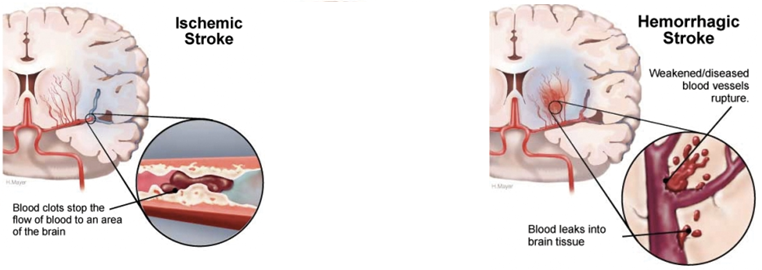
\includegraphics[scale=0.9]{figures/bProblemanalyse/haemoragisk_og_iskaemisk.png}
	\caption{På figuren ses, hvad der sker i encephalon, når hhv. iskæmisk og hæmoragisk apopleksi opstår. Der ses til venstre på billedet, at iskæmisk apopleksi opstår, hvis et blodkar blokeres. Til højre ses, at hæmoragisk apopleksi opstår, når et blodkar brister. \textit{(Revideret)} \cite{Ritter2015}}
	\label{haem-isk}
\end{figure}

\subsubsection{Iskæmisk apopleksi}\label{IskaemiskApp}
Iskæmisk apopleksi opstår i $80$-$85\%$ af alle apopleksitilfælde \cite{Sundhed.dk2014}. Her blokeres et blodkar i encephalon af en blodprop, der stopper tilførslen af blod til et bestemt område, hvilket ses til venstre på \figref{haem-isk}. Blodpropperne dannes primært pga. åreforkalkning enten ved en trombe eller en emboli. En trombe sætter sig fast det sted, hvor den er dannet, og består af blodplader og fibrin. \cite{Schulze2011} En emboli består typisk af fragmenter af blodceller eller kolesterol, som ledes ind i blodkredsløbet til encephalon fra andre blodkar i kroppen. \cite{Academic2015a}.% grundet iltmangel efter få minutter, og hvis dette fortsætter i en periode, vil de til sidst gå tabt. [5] % Specificer denne periode - hvor lang tid går der, før nervecellen går tabt?

\subsubsection{Hæmoragisk apopleksi}
Hæmoragisk apopleksi opstår i $10$-$15\%$ af alle apopleksitilfælde \cite{Sundhed.dk2014}. Årsagen hertil er hovedsagligt forhøjet blodtryk eller, i sjældnere tilfælde, aneurismer eller medfødte misdannede kar \cite{Schulze2011}. Hæmoragisk apopleksi opstår, når en hjernearterie brister, og en lækage af blod danner en blodansamling, hvilket ses til højre på \figref{haem-isk}. Dette øger trykket i encephalon og kan beskadige det omkringliggende væv. \cite{Caplan2006}\\
Intracerebral hæmoragi opstår ofte af forhøjet blodtryk, der danner et pres på de små blodkar, som får dem til at briste. \cite{Caplan2006} Blødning i subaraknoidalrummet skyldes ofte bristning af en aneurisme i encephalon \cite{Schulze2011}.\fxnote{NTK: Subaraknoidalrummene er rummet mellem hjernehinderne} Symptomerne ved subaraknoidalblødning er tab af forskellige hjernefunktioner, da der forekommer et øget pres på cerebrum, hvorimod hæmatomet ved intracerebral hæmoragi er lokaliseret et bestemt sted i encephalon og forårsager nedsat funktion af én bestemt hjernefunktion \cite{Caplan2006}. 

%%%%%%%%%%%%%%%%%%%%%%%%%%%%%%%%%%%%%%%%%%%%%%%%%%%%%%%%%%%%%%%%% Gamle ting
%Apopleksi er af World Health Organization (WHO) defineret som pludseligt opstået fokale neurologiske symptomer pga. forstyrrelser i hjernens blodcirkulation, der varer mere end 24 timer eller fører til døden[1gammel].
% [1gammel] = (Experience from a multicentre stroke register: a preliminary report.): http://www.ncbi.nlm.nih.gov/pubmed?cmd=Search&term=Bull%20WHO%20%5Bta%5D%20AND%2054%5Bvol%5D%20AND%20541%5Bpage%5D 